%% This is an example first chapter.  You should put chapter/appendix that you
%% write into a separate file, and add a line \include{yourfilename} to
%% main.tex, where `yourfilename.tex' is the name of the chapter/appendix file.
%% You can process specific files by typing their names in at the 
%% \files=
%% prompt when you run the file main.tex through LaTeX.
\chapter{The CMS Detector}

\section{Overview}

The Compact Muon Solenoid (CMS) Detector is a general-purpose high-energy physics detector located 100 meters underground in the French side of the LHC \cite{CMSDetector}. Overall, the complete detector is 21 m long, 15 m wide, and 15 m high with a weight of 14 kilotons, heavier than the Eiffel Tower in Paris. It functions as a giant, high-speed camera, taking 3D ``photographs'' of particle collisions from all directions up to 40 million times each second. Figure \ref{CMSRealPic} shows the photo taken for the CMS detector at the underground collision hall.

\begin{figure}[hbtp]
\begin{center}
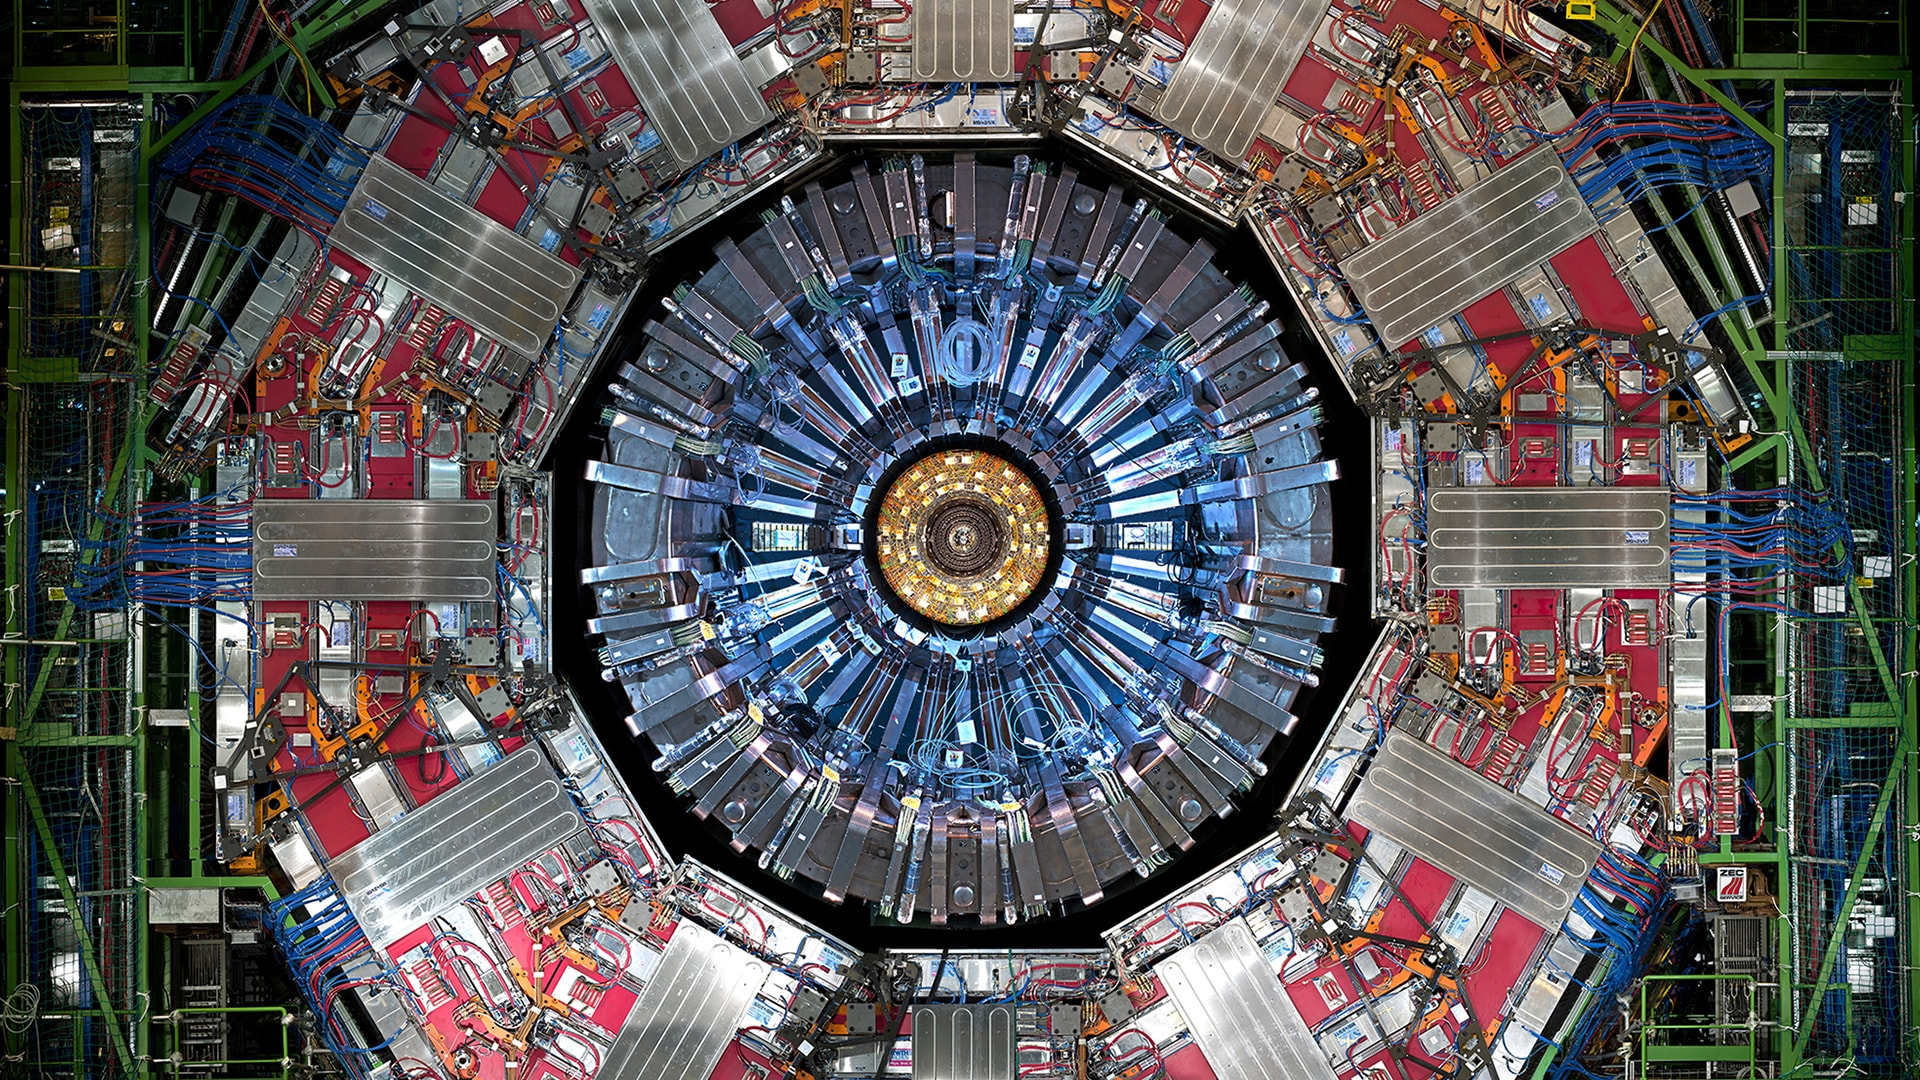
\includegraphics[width=0.80\textwidth]{Figures/Chapter3/CMSRealPic.jpg}
\caption{The front view of the CMS detector at the underground collision hall is shown above.}
\label{CMSRealPic}
\end{center}
\end{figure} 

The CMS detector consists of many sub-detectors including silicon strip and pixel trackers, the pre-shower made of silicon strips, the crystal electromagnetic calorimeter (ECAL), the superconducting solenoid with 3.8 T of magnetic field strength, the inner hadronic calorimeter (HCAL), the steel returning yoke to enhance the magnetic field strength, the outer hadronic calorimeter, the muon chambers, and the forward hadronic calorimeter \cite{CMSDetector}. Figure \ref{CMSDecPic} shows a schematic view of the CMS detector

\begin{figure}[hbtp]
\begin{center}
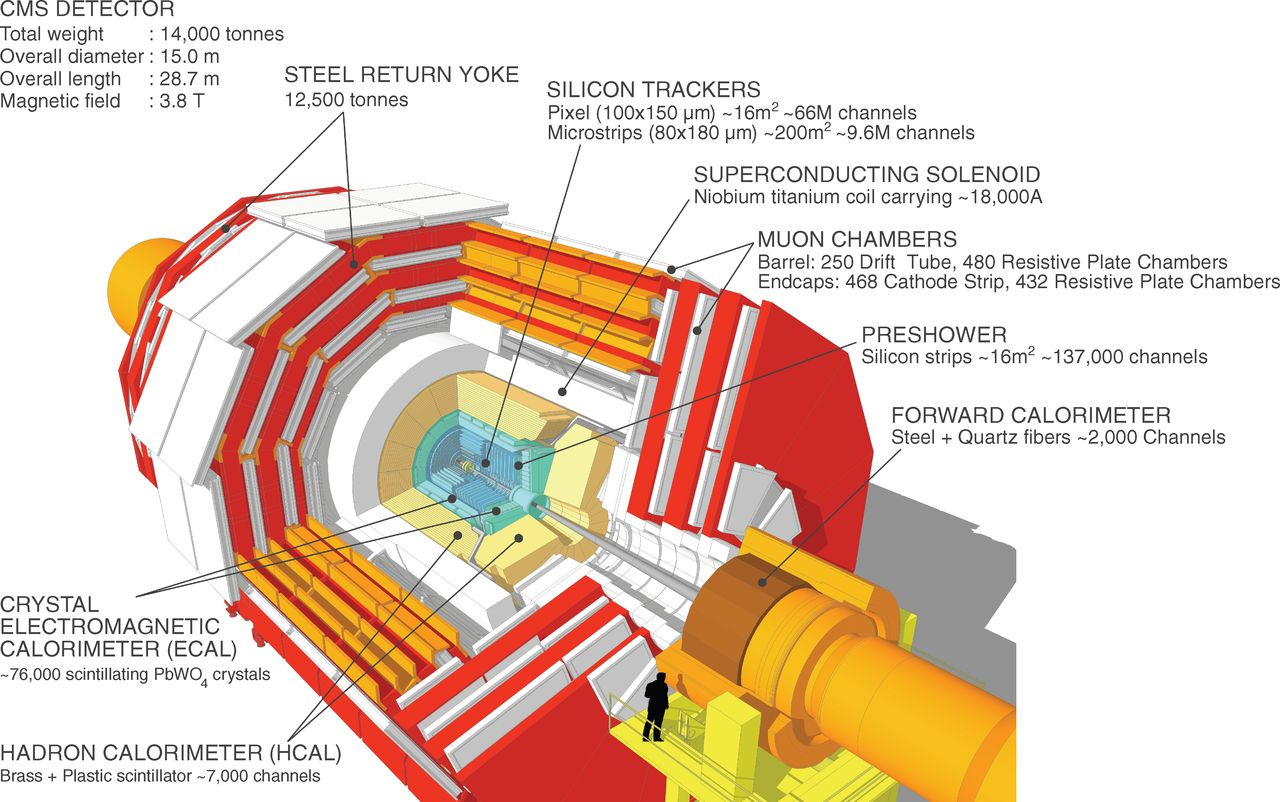
\includegraphics[width=0.80\textwidth]{Figures/Chapter3/CMSDecPic.jpg}
\caption{The schematic view of the CMS detector with brief descriptions of all its components is shown above. Image from \cite{HiggsCMS}}
\label{CMSDecPic}
\end{center}
\end{figure} 

The CMS detector is built, operated, and maintained by the CMS Collaboration. The CMS Collaboration consists of over 4000 members including scientists, engineers, technicians, students, and administrative assistants from 200 institutes and universities in 40 countries around the world. Physicists take data from the CMS detector and share data with each other with the CERN online system, which actually led to the discovery of World Wide Web. The data are store in tapes and kept at different institutions. Members of the CMS experiment collaborate with each other on detector studies and data analysis to produce important scientific results and have published in more than 1000 papers in internationally recognized journals.

In the following sections, I will describe the CMS experiment including the trigger system for data acquisition, the tracking system to track charged particles, the muon system for muon detection, identification, and reconstruction, and the calorimeter system to measure the energies of the particles.

\section{Triggers}

The CMS experiment develops triggers to acquire experimental data \cite{CMSTrigger}. Its main purpose is to select events of potential physics interests from the particles collisions rate of approximately one billion events per second at the LHC. The CMS trigger system consists of two levels of triggers: hardware level 1 (L1) trigger and the software high-level trigger (HLT). Different triggers encoded in the L1 and HLT are designed and fire to collect datasets for specific physics studies.

\subsection{L1 Trigger}

In the CMS experiment, an event is defined as a snapshot of one collision at the LHC. In the L1 trigger, physicists develop algorithms according to detector electronics response to decide if an event is accepted or rejected within the L1 trigger latency time. Figure \ref{L1Overview} shows the schematic overview of the L1 trigger making its decision online to select events based on the information from the calorimeter and muon systems.


\begin{figure}[hbtp]
\begin{center}
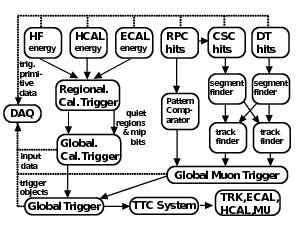
\includegraphics[width=0.50\textwidth]{Figures/Chapter3/L1Overview.png}
\caption{The figure above demonstrates how the CMS L1 hardware trigger function schematically.}
\label{L1Overview}
\end{center}
\end{figure} 

In the interest of heavy-ion studies, physicists develop a set of dedicated triggers algorithms in the L1 trigger to build datasets. The minimum biased (MB) trigger is designed to collect MB data for elliptic flow, $D^0$ mesons, and charged-particle multiplicity analyses while the single muon trigger is designed to select muons events for heavy flavor and electroweak physics analyses. Here, we will explain the MB trigger since we will need to use it to determine the number of MB events in our analysis.

\subsection{MB Trigger}

By definition, an MB event corresponds to a non-single diffractive inelastic interaction \cite{MBTrigger}. A totally inclusive trigger, or called zero bias (ZB) trigger, corresponds to a randomly readout from the detector whenever a collision is possible. MB trigger is an algorithm to determine interesting MB events based on the response from forward HCAL located at $3 < |\eta| < 5$. It puts a fixed analog to digital converter (ADC) threshold in the HCAL response to reject background noise and collect MB events from the ZB trigger. There is also an essentially linear relationship between the maximum ADC with the actual energy response of the forward HCAL. Figure \ref{HFADC} shows the ADC distribution and HF energy as a function of ADC in the 2018 PbPb run.

\begin{figure}[hbtp]
\begin{center}
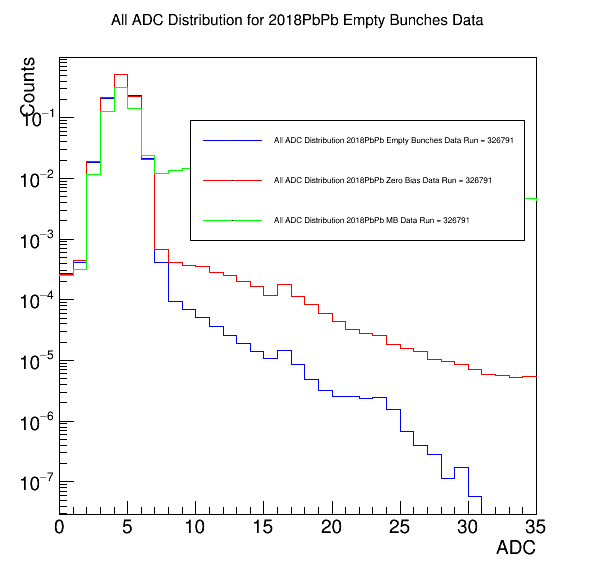
\includegraphics[width=0.45\textwidth]{Figures/Chapter3/AllADC.png}
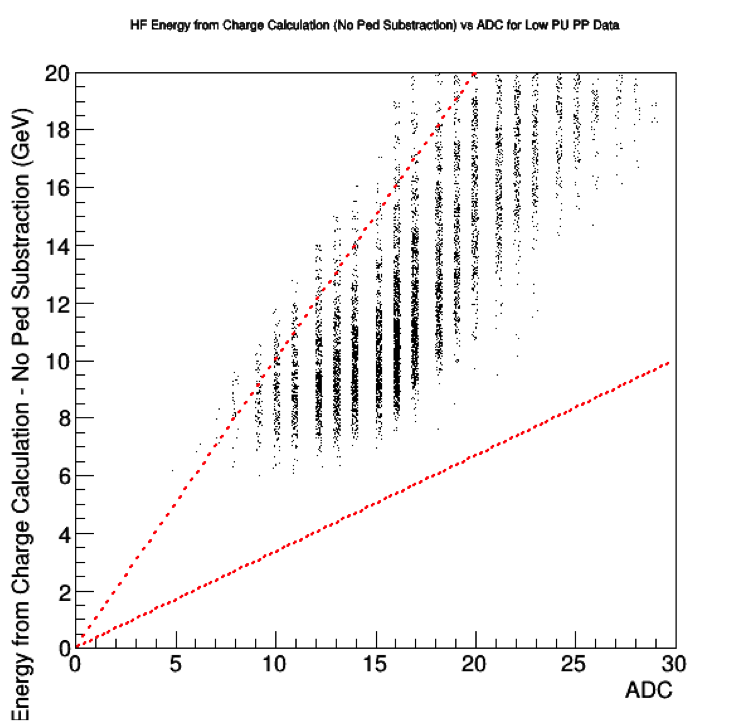
\includegraphics[width=0.45\textwidth]{Figures/Chapter3/HFvsADC.png}
\caption{In the CMS 2018 PbPb Run 326791, the ZB data (red), Empty Bunches (blue), and MB data (green) ADC distributions (left) and the HF energy according to the charges collected as a function of ADC (right) are shown above. We can see that the HF energy has conversion factor about (0.5 - 1) to the ADC.}
\label{HFADC}
\end{center}
\end{figure} 

The MB trigger consists of ``MB OR'', which requires the ADC thresholds on either one of the forward HCAL (HF) out of both forward ECAL in both positive and negative sides, and ``MB AND'',  which requires the ADC thresholds on both of HFs out of both forward ECAL in both positive and negative sides. Figure \ref{2018PbPbMB} shows the L1 MB trigger analysis of Run 326791 in the 2018 CMS PbPb data taking 

\begin{figure}[hbtp]
\begin{center}
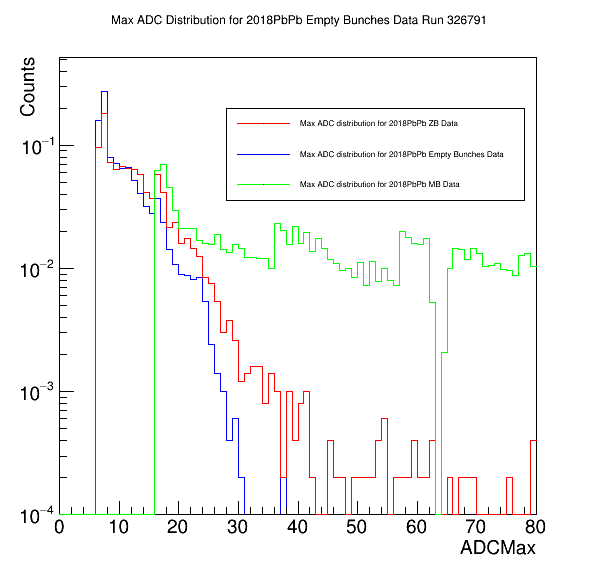
\includegraphics[width=0.45\textwidth]{Figures/Chapter3/MaxADC.png}
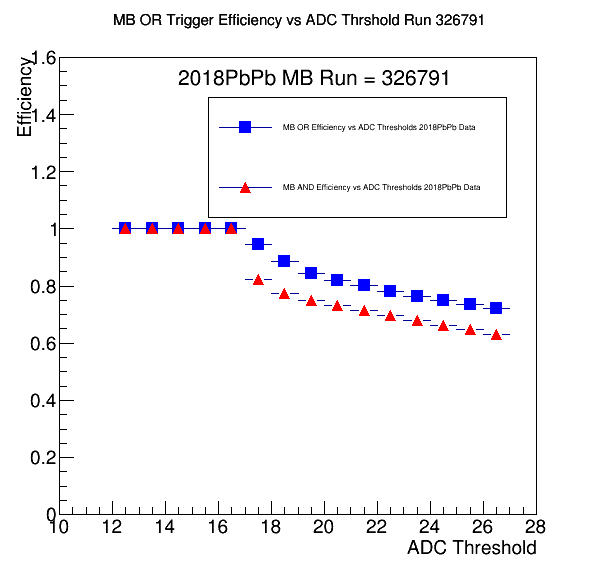
\includegraphics[width=0.45\textwidth]{Figures/Chapter3/MBTrgEffADC.png}
\caption{In the CMS 2018 PbPb Run 326791, the ZB data (red), Empty Bunches (blue), and MB data (green) maximum ADC distributions (left) and the efficiencies of MB OR (blue) and MB AND (red) as a function ADC threshold (right) are shown above.}
\label{2018PbPbMB}
\end{center}
\end{figure} 

In the 2018 CMS PbPb data taking, to reject the noisy background, the max ADC of each event is required to be greater than 15 with MB AND along with the HLT trigger. In addition, at least 1 pixel track are applied to select MB events, as seen above from Figure \ref{2018PbPbMB} in the max ADC distribution of MB events in green. A total number of about 2.4 billion MB events corresponding to a luminosity of about 1.7 $nb^{-1}$ have been collected by CMS during the 2018 LHC PbPb run from November to December 2018. Figure \ref{MBStat} shows the MB events and corresponding luminosity as a function of Runs ID throughout the 2018 CMS PbPb data-taking period

\begin{figure}[hbtp]
\begin{center}
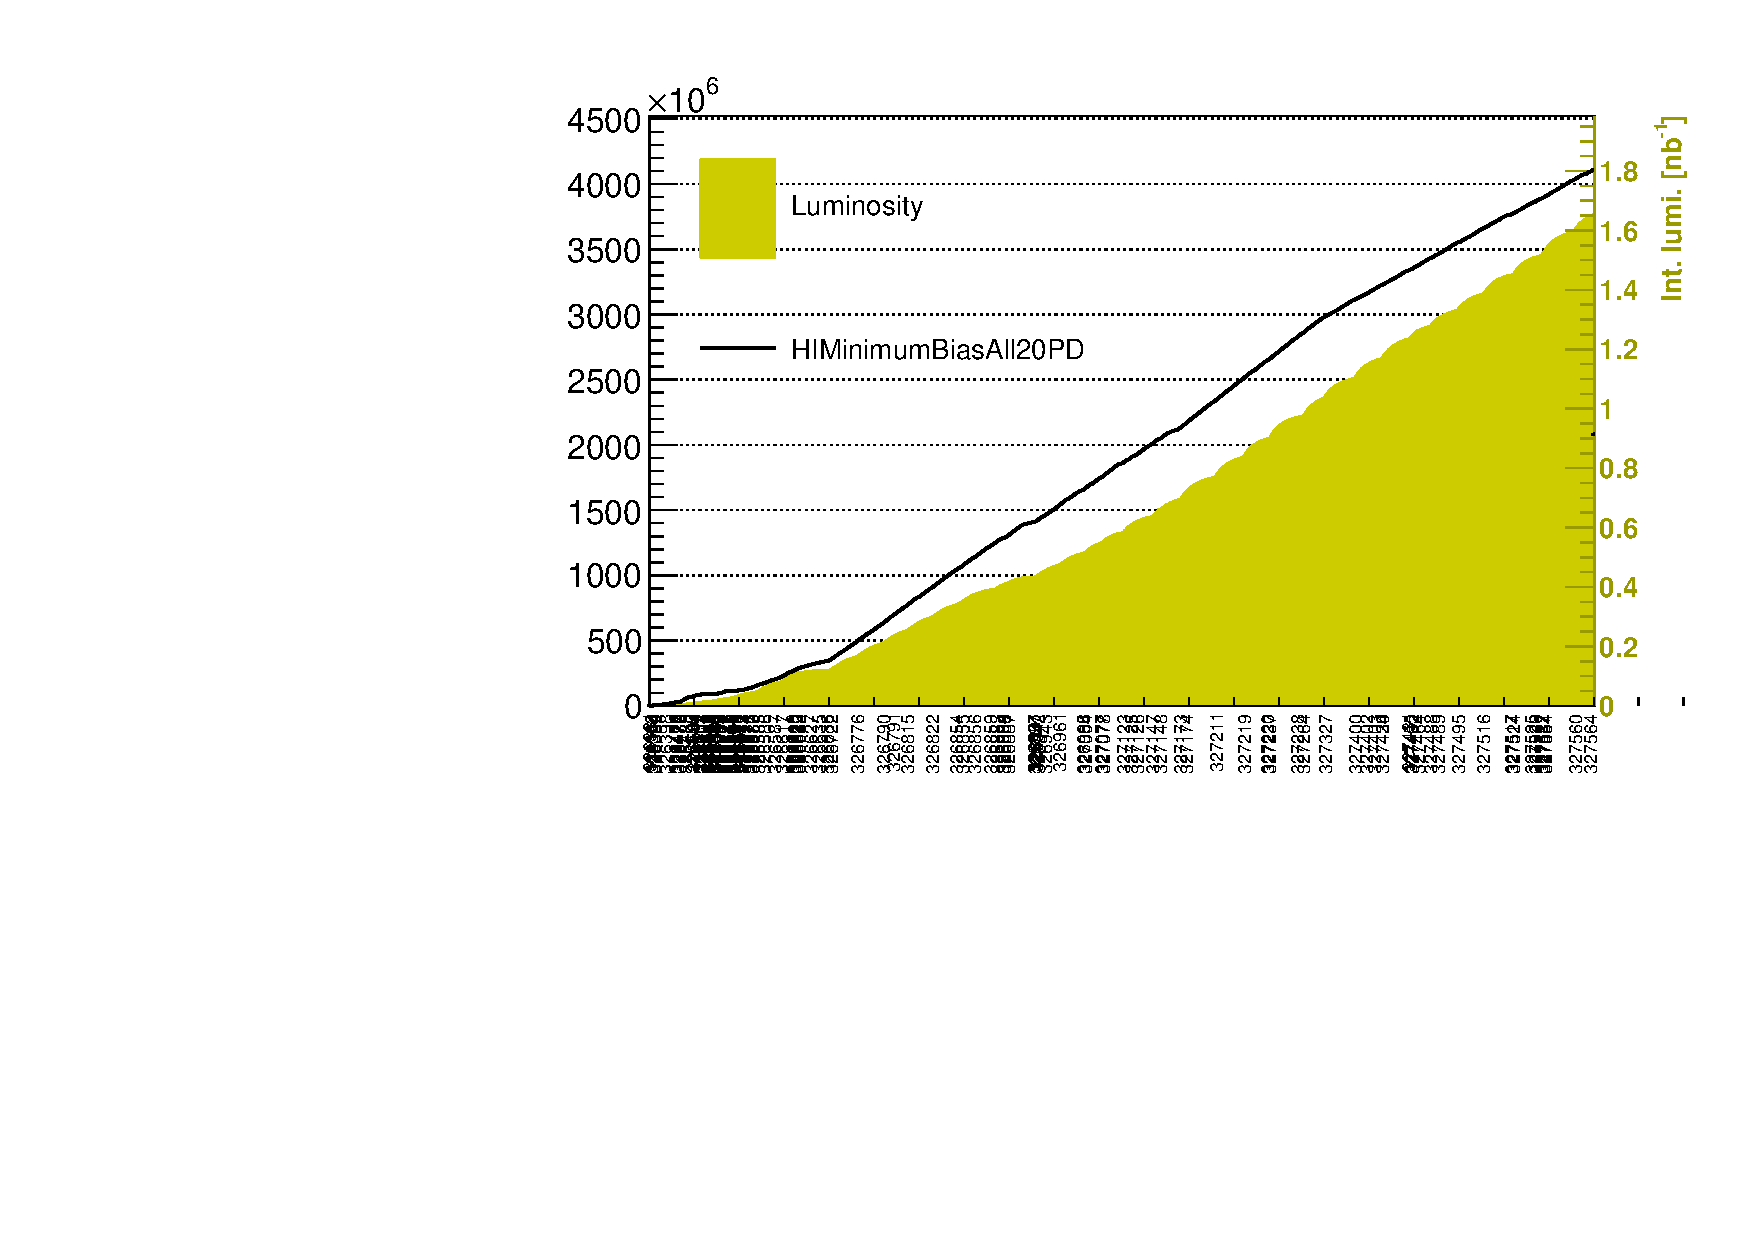
\includegraphics[width=0.55\textwidth]{Figures/Chapter3/MBStat.pdf}
\caption{The figure above shows the total number of 20 PbPb MB events from and corresponding luminosity how the as a function Run ID from November 15 to December 2, 2018.}
\label{MBStat}
\end{center}
\end{figure} 


\subsection{Centrality Efficiency with MB Trigger}

In addition to overall efficiency vs the ADC with the MB trigger, we also study the centrality efficiency with different ADC thresholds. Figure \ref{EffCent} shows the centrality as a function of efficiency using MB OR and MB AND with different thresholds

\begin{figure}[hbtp]
\begin{center}
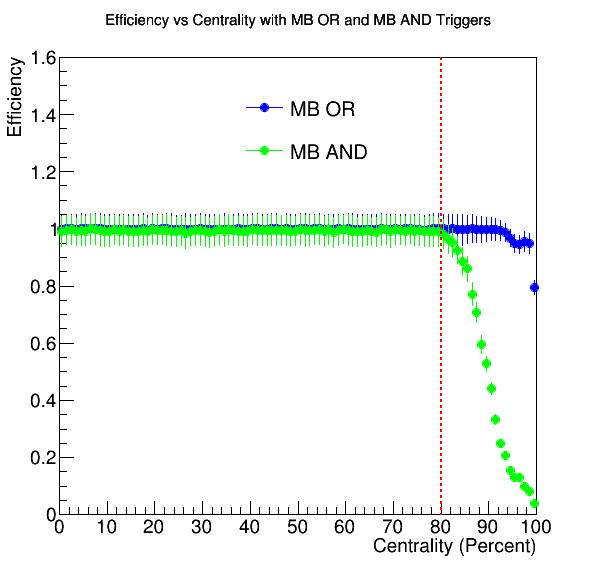
\includegraphics[width=0.55\textwidth]{Figures/Chapter3/EffCent.png}
\caption{The efficiency vs centrality with ADC > 16 for MB OR (blue) and MB AND (green) are shown above.}
\label{EffCent}
\end{center}
\end{figure} 

Because other physics triggers are mainly based on the MB datasets, in the physics analyses using 2018 CMS PbPb datasets, it is recommended to remove the very peripheral centrality range from 90 - 100\%, which is not fully efficient (efficiency $<$ 100\%). Therefore, most of the CMS heavy-ion physics results using the 2018 PbPb dataset will be reported in the centrality range of 0 - 90\%.

\subsection{HLT Trigger}

The HLT software trigger is an array of commercially available computers running high-level physics algorithms \cite{CMSTrigger}. Unlike the online L1 hardware trigger which runs on-the-go during the data-taking process, HLT is an offline software trigger that runs after the data are acquired. In the HLT trigger, more sophisticated analyses are performed to determine if the event is kept or not for a specific dataset. The event data are stored locally on disks and eventually transferred to downstream systems, the CMS Tier-0 computing center, for offline HLT processing and permanent storage \cite{CMSTrigger}. Many trigger paths in the HLT, such as the high multiplicity trigger to specifically collect events with many tracks, the D-meson trigger to select high $p_T$ D mesons, and the dimuon trigger to enrich Drell-Yen events, are designed and encoded in the HLT trigger. In the following, we will describe the dimuon trigger in detail because the dimuon dataset will be used to fully reconstruct B mesons in this thesis. 

\subsection{DiMuon Trigger}

The dimuon trigger, as it is named, is a trigger based on the information of two muons tracks. The HLT is able to quickly reconstruct the invariant mass of two oppositely charged muons $m_{\mu\mu}$. Figure \ref{DimuonInvMass} shows the $m_{\mu\mu}$ reconstructed by the CMS HLT with the 2018 $pp$ dataset.

\begin{figure}[hbtp]
\begin{center}
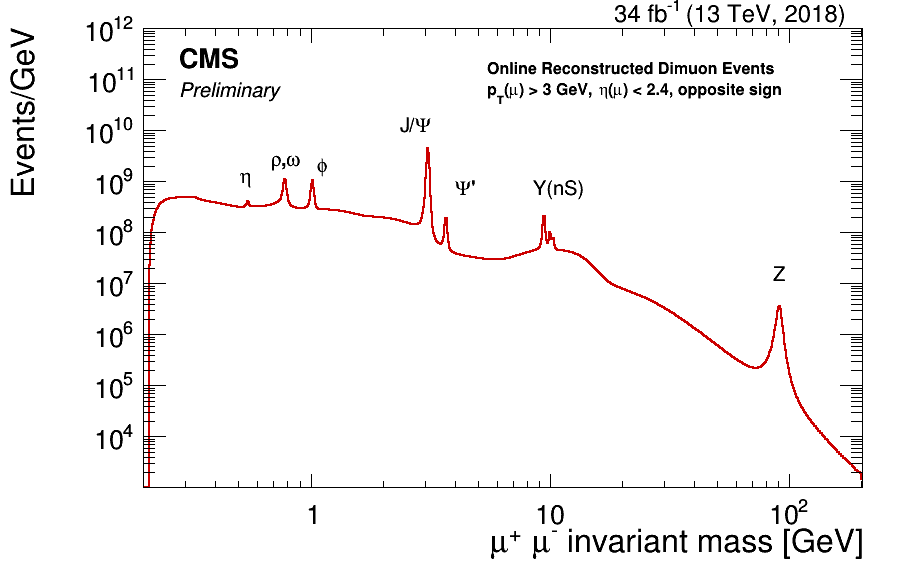
\includegraphics[width=0.55\textwidth]{Figures/Chapter3/DimuonInvMass.png}
\caption{The dimuon invariant mass spectrum $m_{\mu\mu}$ reconstructed by CMS HLT trigger in the 2018 $pp$ dataset is shown above. We can identify the neutral vector boson resonances above.}
\label{DimuonInvMass}
\end{center}
\end{figure} 


In the 2018 PbPb run, the dimuon trigger requires the presence of two muon candidates, with no explicit momentum threshold and with the HLT reconstructed dimuon invariant mass of 1.0 GeV/c$^2$ $< m_{\mu\mu} <$ 5.0 GeV/c$^2$, near the $J/\psi$ PDG mass $m_{J/\psi} =$ 3.0969 GeV/c$^2$ \cite{AlphaTheoEx}, in coincidence with lead bunches crossing at the interaction point. Moreover, one of the trigger-level muons is reconstructed using information both from the muon detectors and the inner tracker with the requirement of more than or equal to 10 hits (named as L3 muon), while the other one muon only requires information from the muon detectors (named as L2 muon) \cite{BAnaDimuonTrigger}.

\section{Tracking System}

\subsection{Silicon Detectors}

The CMS tracking system applies solid-state semiconductor technologies. It consists of the 3 layers of silicon pixel tracker and 10 layers of silicon strip detector including 4 inner barrel layers and 6 outer barrel layers \cite{CMSSilicon}. It has a $\phi = 2\pi$ and $|\eta| < 2.4$ acceptance coverage. Figure \ref{CMSTracker} shows the CMS tracking system schematically

\begin{figure}[hbtp]
\begin{center}
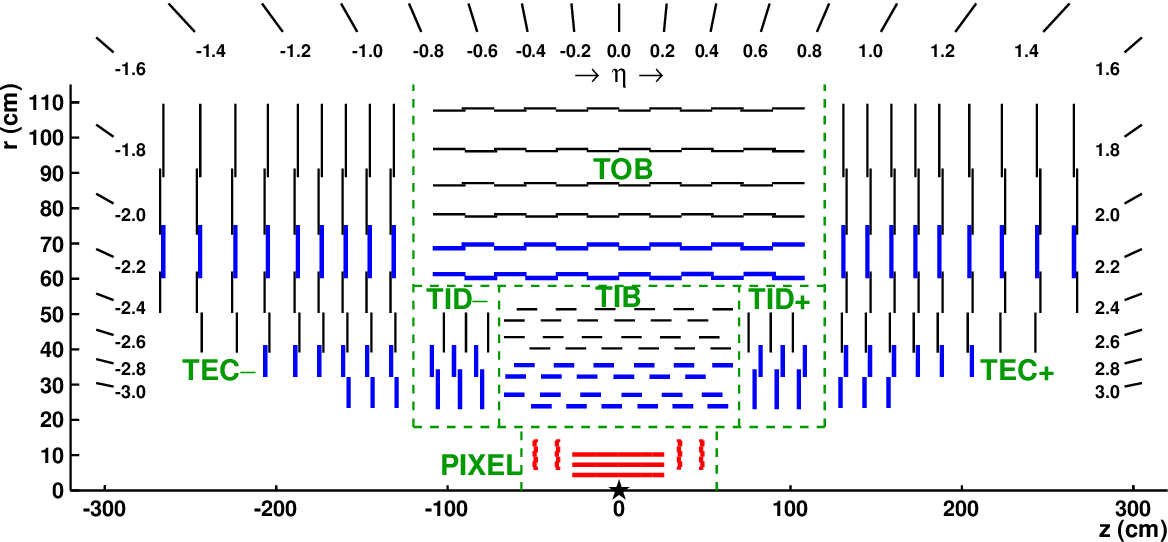
\includegraphics[width=0.80\textwidth]{Figures/Chapter3/CMSTrackingSchemtic.png}
\caption{The schematic view of the CMS tracking system is shown above.}
\label{CMSTracker}
\end{center}
\end{figure} 


In nuclear and particle physics, a tracker is a detector that measures the trajectories of charged particles via ionization. In general, it does not destroy or significantly change the energy of the particle. With the external magnetic field, the tracker can measure the momentum, the charge, and the mass of the particle by studying the electric charges collected from electron avalanches or electron-hole pairs. The CMS tracking systems provide physicists with excellent tracking capabilities. The CMS silicon tracker is a solid-state detector employing semiconductor technologies. The silicon tracker is operated at a reserve bias mode with a depletion voltage of about 600V. A high energy charged particle passing through the silicon tracker have an energy loss of $dE/dx \simeq 0.5$ keV/$\mu$m \cite{AlphaTheoEx}. Therefore, for a 320 $\mu m$ thick silicon sensor, the charged particle will lose about 160 keV. The electron-hole pair in silicon is about 3 eV per pair. Therefore, the charged particle will produce roughly on the order of $10^4$ electrons. The hit resolution in $r\phi$ direction of the silicon strip is about 10 -- 40 $\mu m$ \cite{CMSTrackComp}. Figure \ref{SiliconDetector} shows schematically how a high-energy charged particle ionizes an electron-hole pair in the depletion region of a silicon P-N junction diode operated at a reverse-bias mode


\begin{figure}[hbtp]
\begin{center}
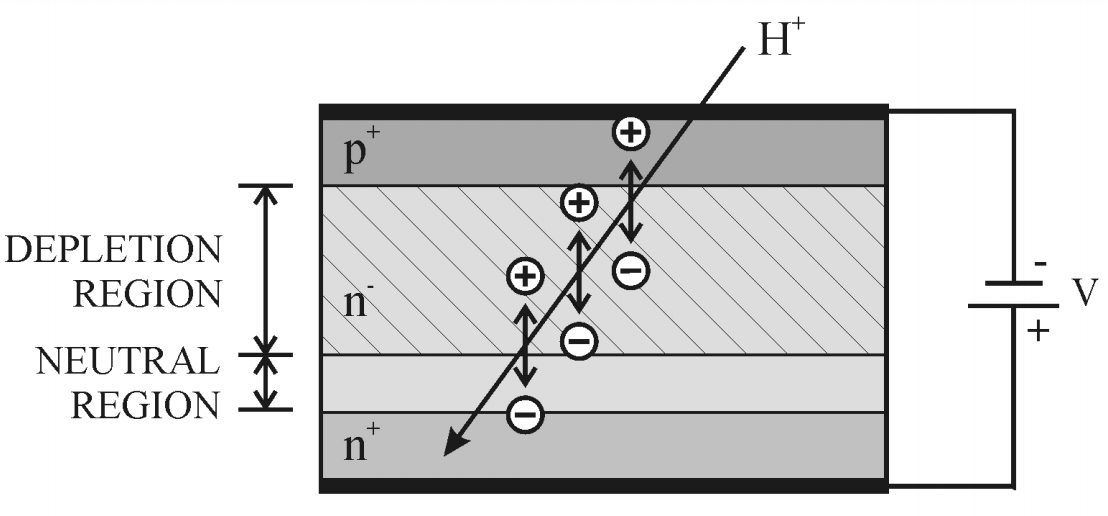
\includegraphics[width=0.75\textwidth]{Figures/Chapter3/SiliconDetector.png}
\caption{The schematic plot explaining how a silicon tracker detects charged particles is shown above.}
\label{SiliconDetector}
\end{center}
\end{figure} 

However, in the CMS silicon tracker, due to the small number of electrons produced in the silicon sensors, the energy loss $dE/dx$ as a function of momentum $p$ of charged particles does not have sufficiently good resolution to separate and identify electron, pion, kaons, and protons. Therefore, we generally do not perform particle identification (PID) for hadrons with the CMS detector in physics analyses.  

\iffalse

\subsection{Tracking Algorithm}

With the hardware silicon tracker, the CMS collaboration also developed the state-of-the-art tracking algorithm to reconstruct the paths and primary vertices of the collisions from the electronic readout signals. CMS tracking algorithm employs the Combinatorial Track Finder (CTF), an adaptation of the combinatorial Kalman filter \cite{CMSTrack1,CMSTrack2,CMSTrack3}, which in turn is an extension of the Kalman filter \cite{Kalman} to allow pattern recognition and track fitting to occur in the same framework. The collection of reconstructed tracks is produced by multiple passes (iterations) of the CTF track reconstruction sequence, in a process called iterative tracking \cite{CMSTrackComp}. The CMS tracking workflow and its performance are shown in Figure \ref{TrackWorkFlow} and Figure \ref{CMSTrackPer}

\begin{figure}[hbtp]
\begin{center}
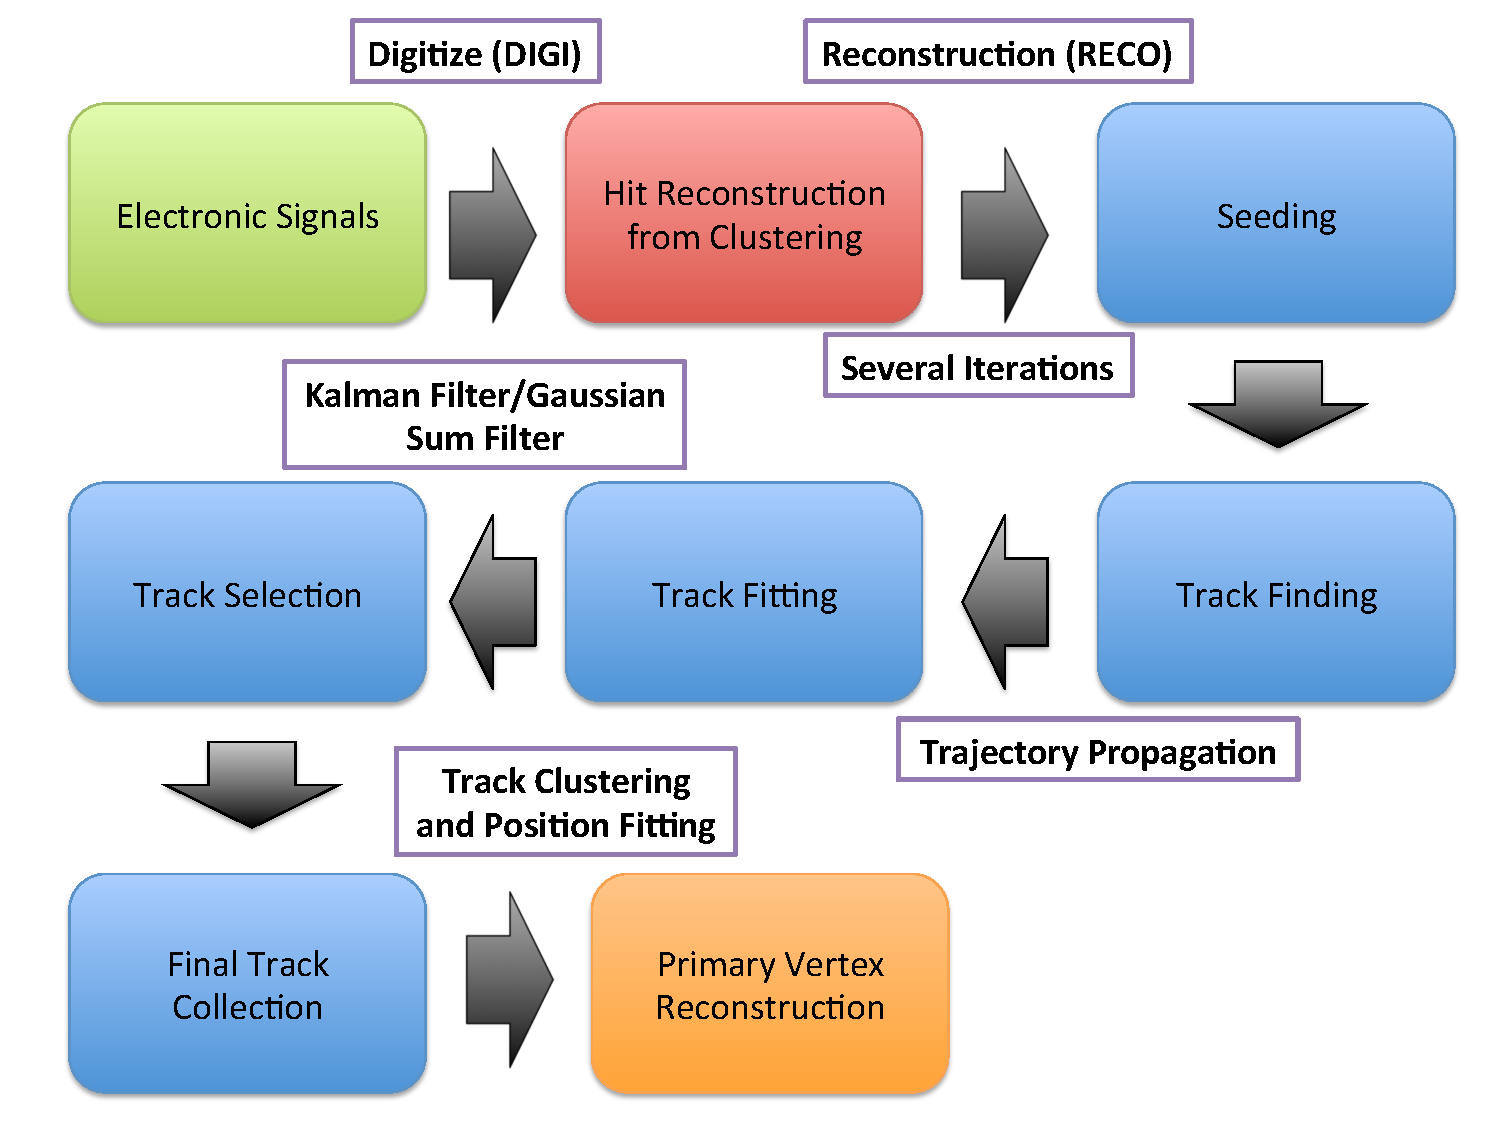
\includegraphics[width=0.90\textwidth]{Figures/Chapter3/TrackWF.pdf}
\caption{The schematic block diagram of CMS tracking workflow is shown above.}
\label{TrackWorkFlow}
\end{center}
\end{figure} 


%Figure \ref{CMSTrackPer} shows the general performance of CMS tracking algorithm

\begin{figure}[hbtp]
\begin{center}
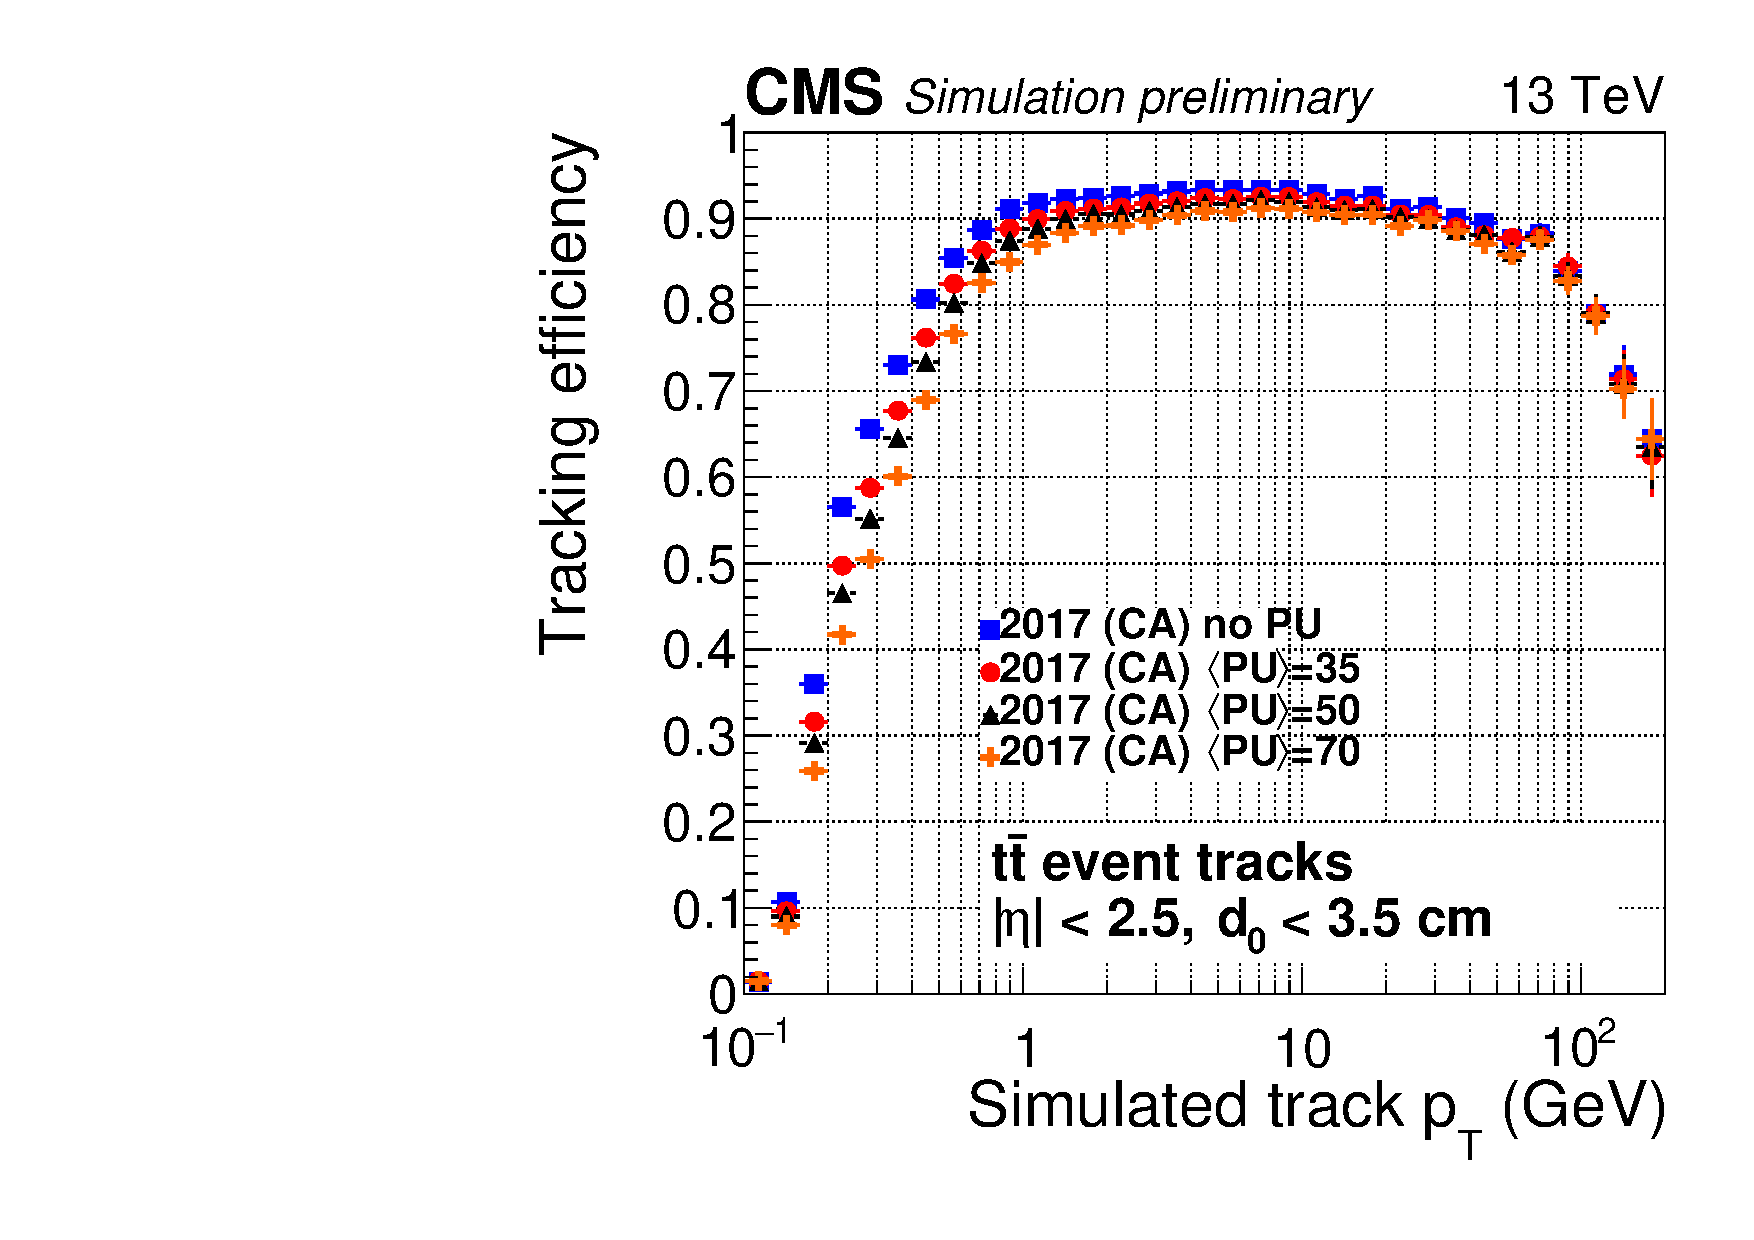
\includegraphics[width=0.48\textwidth]{Figures/Chapter3/TrackPTEff.pdf}
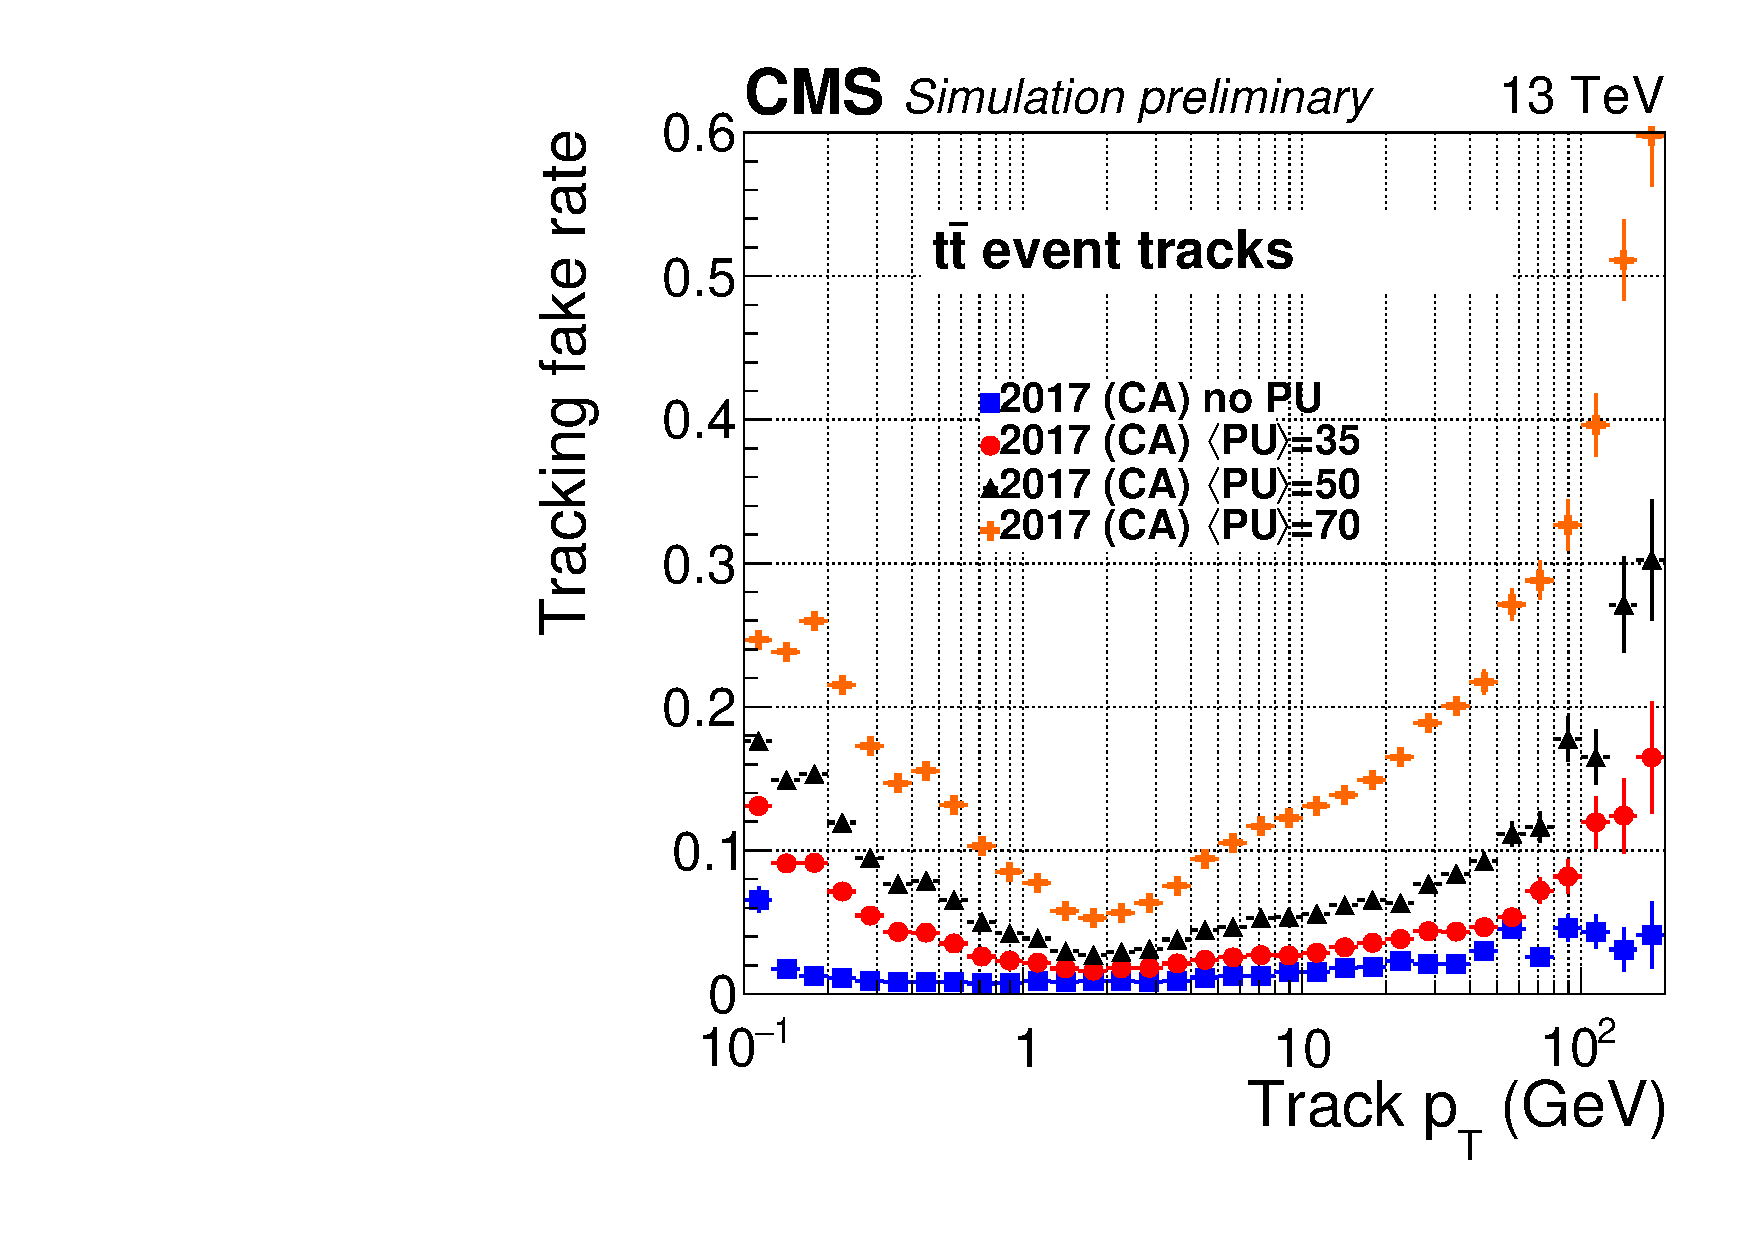
\includegraphics[width=0.48\textwidth]{Figures/Chapter3/TrackPTFake.pdf}
\caption{The CMS tracking efficiency (left) and fake rate (right) as a function of $p_T$ from simulations of $t \bar t$ events at 13 TeV with different pileup conditions are shown above.}
\label{CMSTrackPer}
\end{center}
\end{figure} 

Finally, with the collection of tracks, assuming all the tracks are promptly produced at a given interaction point, we can determine the primary vertex by selecting the tracks, performing track clustering, and fitting for the position of each vertex using its associated tracks \cite{CMSTrackComp}. The deterministic annealing algorithm \cite{DAAlgo} is track clustering algorithm that CMS is currently using. The track and vertex information of each event will be stored in datasets for physics analyses.

\fi

\section{Muon System}

Named as the ``Compact \textbf{Muon} Solenoid'', the muon capability is one of the most important features of the CMS experiment. The CMS muon system, with an acceptance coverage of $|\eta| < 2.4$, has 1400 muon chambers including 250 drift tubes and 540 cathode strip chambers to track the positions of the muons and provide a trigger. Its 610 resistive plate chambers form a redundant trigger system. Due to the small energy loss of muon in ECAL and HCAL \cite{AlphaTheoEx}, the muons produced from the LHC usually penetrate through the trackers and calorimeters. Therefore, the muon system is located at the outermost of the CMS detector. Figure \ref{ParticleFlow} shows the particles produced at the interaction points and pass through the CMS detector

\begin{figure}[hbtp]
\begin{center}
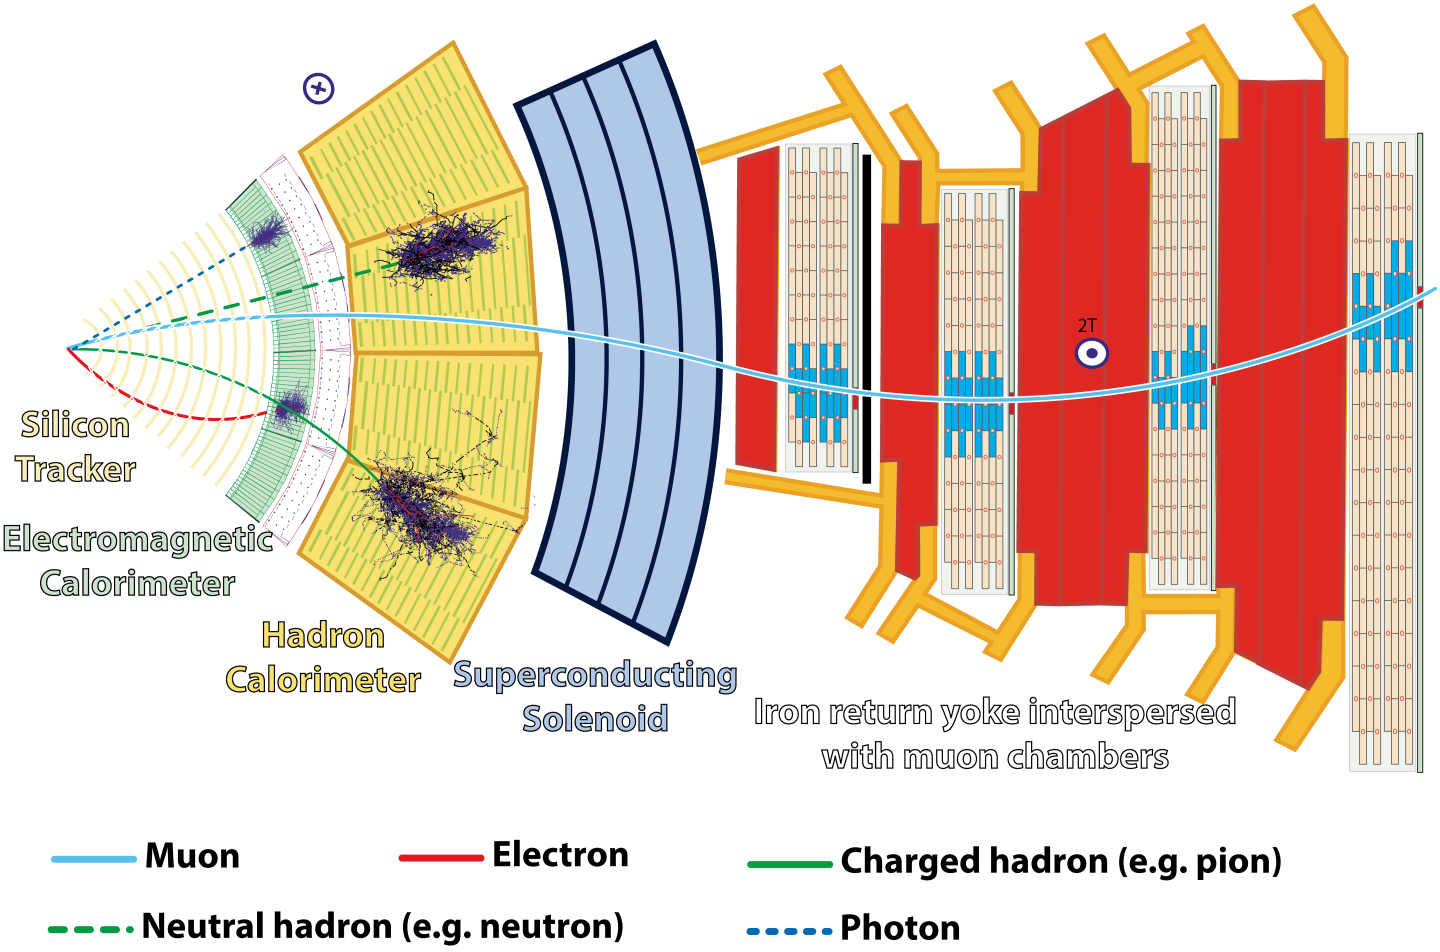
\includegraphics[width=0.90\textwidth]{Figures/Chapter3/CMSParticleFlow.png}
\caption{The particle flow of long-life particles, such as electrons, muons, photons, charged hadrons: $\pi,K,p$, and neutral hadrons: neutrons, in the CMS detector are shown above.}
\label{ParticleFlow}
\end{center}
\end{figure} 

%\textbf{How MUON CHAMBER WORKS}

The muon system employs gaseous detector technology. The physical modules of drift tubes, cathode strip proportional planes, and resistive plates are called ``chambers''. When a muon passes through the chambers, it will ionize electrons of the gas atoms. Under a strong electric field, the avalanche electrons will be drifted to the anode and the gas ion will be drifted to the cathode. An electronic signal will be generated as this occurs. Figure \ref{Muonsystem} shows schematically how electron avalanches work in a gaseous detector to detect charged particles as well as the design of CMS drift tube to detect muons.


\begin{figure}[hbtp]
\begin{center}
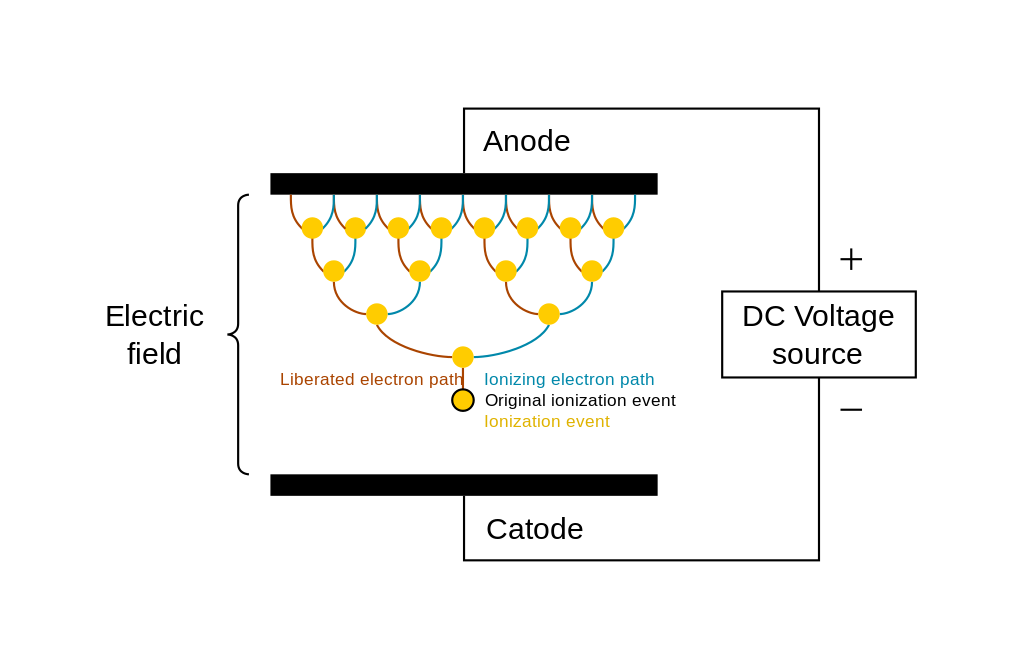
\includegraphics[width=0.85\textwidth]{Figures/Chapter3/EAva.png}
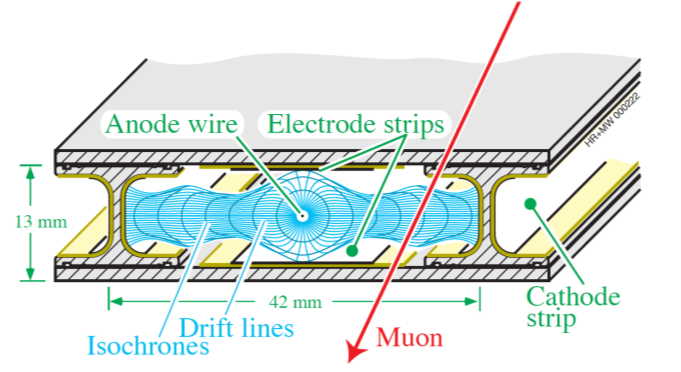
\includegraphics[width=0.85\textwidth]{Figures/Chapter3/CMSDT.png}
\caption{A visualization of Townsend Avalanche (top) and schematic plot of the CMS drift tube detecting a muon (bottom) are shown above.}
\label{Muonsystem}
\end{center}
\end{figure} 


%The muon in the tracker uses a similar tracking algorithms as other charged particles \cite{CMSTrackComp}. Muon tracking performance is excellent. For isolated muons with 1 < $p_T$ < 100 GeV/c, the tracking efficiency is $>$ 99\% over the full $\eta$-range of tracker acceptance and does not significantly depend on $p_T$ while the fake rate is negligible \cite{CMSTrackComp}. We can require hits on the outer most muon chambers to identify muons because other charge particles will be stopped by the calorimeter and should not be able to enter the muon system as shown on Figure \ref{ParticleFlow}. Therefore, the CMS muon system has excellent capabilities of detecting, identifying, and reconstructing muons, which is crucial for heavy flavor physics studies. 

Therefore, with both the tracking system and the muon chambers, the CMS detectors have excellent capabilities of detecting, identifying, and reconstructing muons, which is crucial for heavy flavor physics studies.

\section{Calorimeter System}

In nuclear and particle physics, a calorimeter is a detector that completely stops particles and measures the total energy deposited. According to the particles, the calorimeters can be divided into electromagnetic calorimeters (ECAL or EMCAL) to measure the energy of electrons and photons and hadronic calorimeters to measure the energy of charged and neutral hadrons. The CMS calorimeter system includes both ECAL and HCAL. It is located in between the tracker and the muon chambers as shown in Figure \ref{CMSDecPic}. 

According to the measurement of the shower energy, calorimeters can typically be classified as sampling calorimeters and homogenous calorimeters. The sampling calorimeters have two components: absorber and scintillator. The absorber is generally made of metals and produces the shower. The scintillator collects a fraction of the total energy from the shower (visible energy) and then corrects the visible energy back to the total energy based on the light collection efficiency. On the other hand, the homogenous calorimeters collect all the energy deposited. Their materials producing the particle shower also measure energy deposition. 

\subsection{ECAL}

The CMS ECAL is made of lead tungstate (PbWO$_4$) crystal and is a homogeneous type calorimeter. High energy electrons and photons interact with the CMS ECAL and undergo bremsstrahlung to produce electrons, positrons, and photons and deposit energy to the ECAL. It has an acceptance coverage of $|\eta| < 1.48$ with a high granularity of $\Delta \eta \times \Delta \phi = 0.0175 \times 0.0175$ in the barrel region and 1.5 $< |\eta| <$ 3.0 in the endcap region. In addition, the ECAL has an excellent energy resolution of $\frac{\Delta E}{E} = \frac{2.83\%}{\sqrt {E}} \oplus \frac{12.0\%}{E}  \oplus 0.26\%$ where $E$ is in the unit of GeV \cite{ECALReso} to precisely measure the energy of electrons and photons. It is capable of identifying electrons and detecting photons, which is crucial for heavy flavor physics studies and photon-jet analysis. 

\subsection{HCAL}

The CMS HCAL is a sampling type calorimeter made of 926 tons of steel or brass. Over a million World War II brass shell casements are from the Russian Navy. Hadrons interact with the HCAL brass and steel nuclei and produce hadronic showers. A fraction of the shower energy is sampled by the tiles of plastic wavelength shifting scintillators and transferred readout boxes. Generally, particles, except muons and neutrinos, will not be able to penetrate the HCAL. The CMS HCAL system consists of the inner HCAL with barrel (HB) and endcap (HE), the outer HECAL (HO), and the forward HCAL (HF). The acceptance coverages of HB, HE, and HO are $|\eta| < $1.39, $|\eta| < $1.26, 1.31 $< |\eta| < $3.0, and 2.85 $< |\eta| < $5.19 respectfully. The HO and HB have a granularity of $\Delta \eta \times \Delta \phi = 0.087 \times 0.087$. The overall energy resolution of HCAL is $\frac{\Delta E}{E} \approx \frac{100\%}{\sqrt {E}}$ \cite{HCALReport}, which is excellent for jet physics studies.

\subsection{HF}

The forward HCAL is a special component of the CMS HCAL system. It is segmented into 36 $\times$ 13 towers in the $\eta - \phi$ plane. Figure \ref{HFPic} shows schematic and physical views of the CMS HF detector \cite{HFInfo}

\begin{figure}[hbtp]
\begin{center}
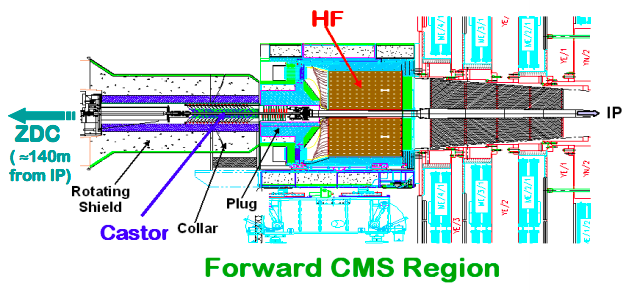
\includegraphics[width=0.58\textwidth]{Figures/Chapter3/CMSForwardRegion.png}
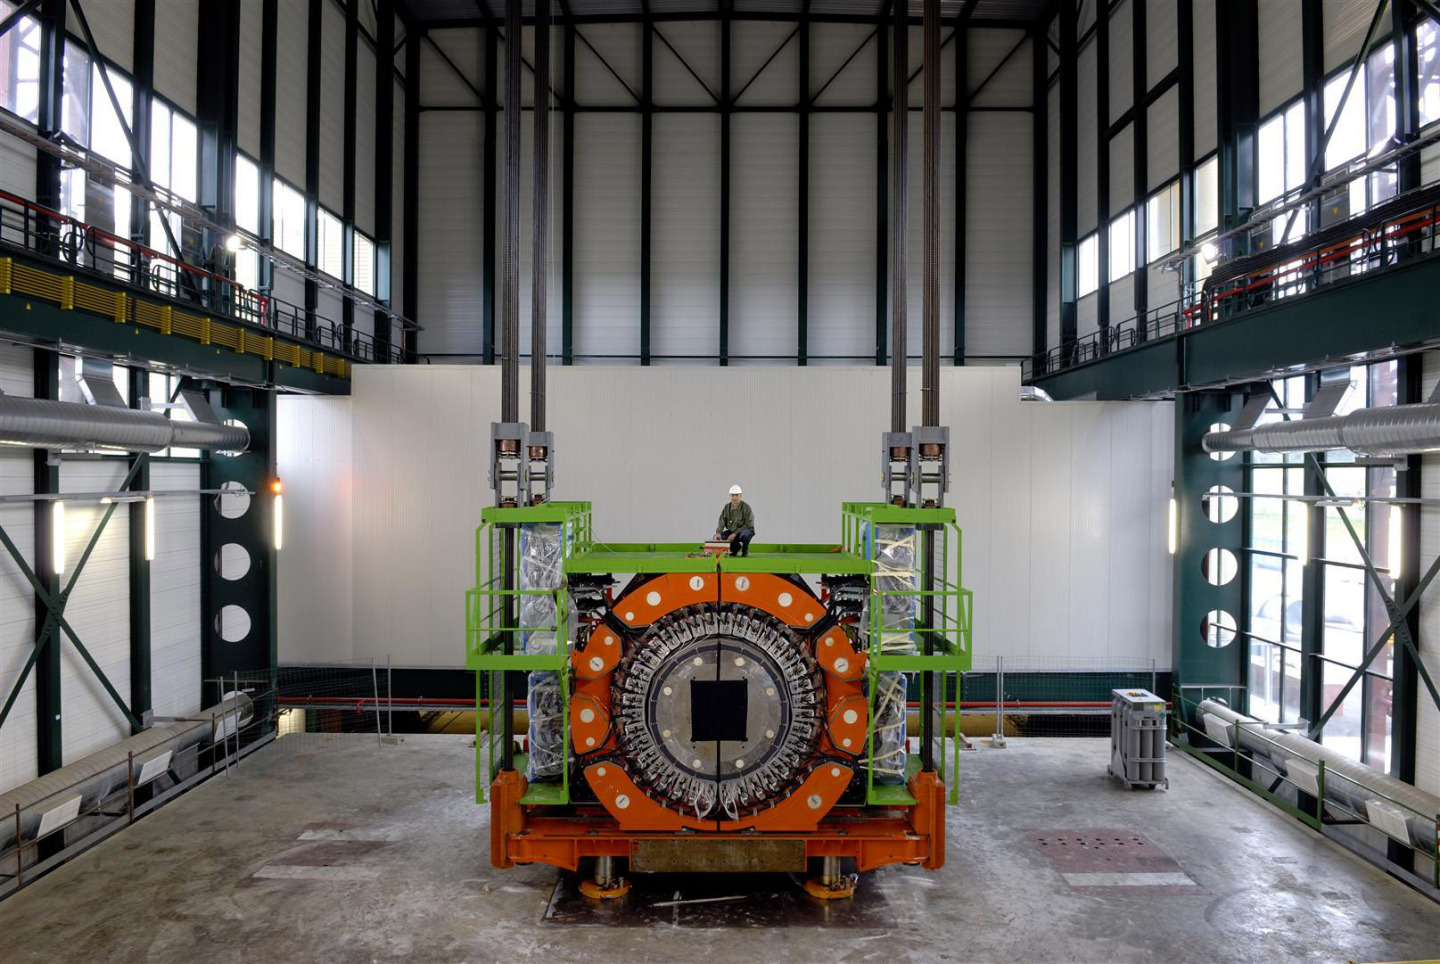
\includegraphics[width=0.38\textwidth]{Figures/Chapter3/HFReal.jpg}
\caption{The schematic view of the CMS forward region including HF, CASTOR, and ZDC (left) and the physical view of the HF (right) are shown above.}
\label{HFPic}
\end{center}
\end{figure} 

As mentioned above, we have developed the L1 MB trigger based on the HF response to select MB events. In addition, in CMS, centrality is defined based on the activities in the HF \cite{HFCentRef}. The more activities are there in the HF, the more remnants of colliding nuclei, the more central the collision event is. Figure \ref{HFCent} shows the determination of centrality range from the HF response 



\begin{figure}[hbtp]
\begin{center}
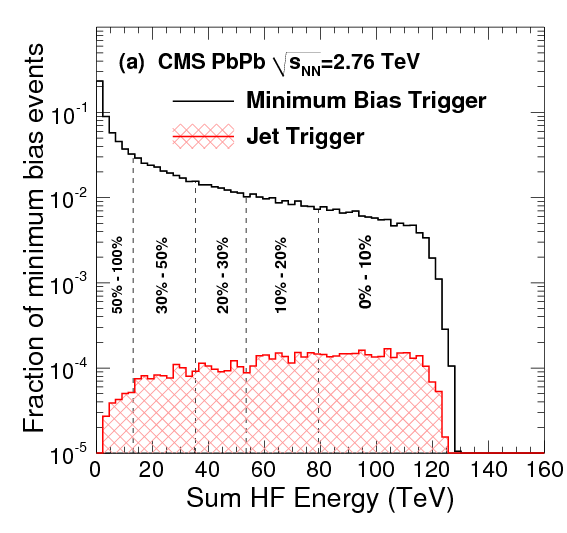
\includegraphics[width=0.70\textwidth]{Figures/Chapter3/HFCent.png}
\caption{The distribution of the sum of HF energy using MB Trigger and Jet Trigger with the classification of centrality binning is shown above. As we can see, the energy of the HF increase as the collision events become more central, which  is within our expectation.}
\label{HFCent}
\end{center}
\end{figure} 



In addition to HF, CASTOR ($-$6.6 $< \eta <$ $-$5.2) and ZDC ($|\eta|$ > 8.1) are also calorimeters located at the very forward region \cite{CASZDCRef} as shown above in Figure \ref{HFPic}. They can help select MB events and trigger ultra-peripheral collision (UPC) events. Figure \ref{CASTORZDC} shows the pictures of CASTOR and the ZDC in the very forward direction of the CMS detector

\begin{figure}[hbtp]
\begin{center}
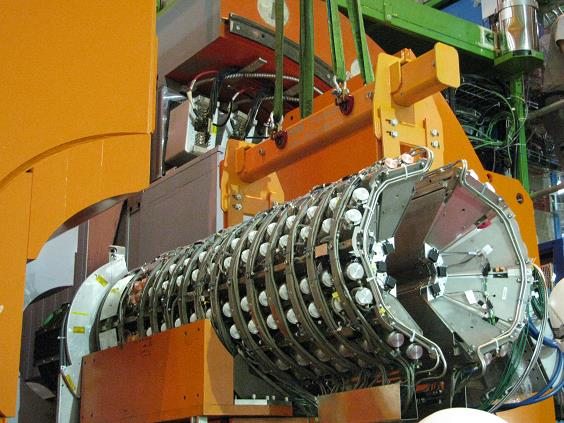
\includegraphics[width=0.44\textwidth]{Figures/Chapter3/CASTOR.png}
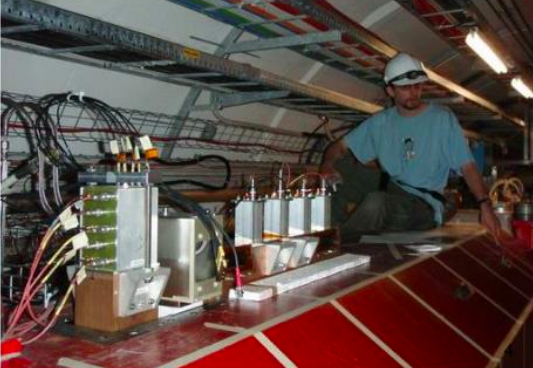
\includegraphics[width=0.50\textwidth]{Figures/Chapter3/CMSZDC.png}
\caption{The picture of the CASTOR (left) at the CMS underground collision hall and ZDC (right) at 140 m away from the CMS beam interacting point are shown above.}
\label{CASTORZDC}
\end{center}
\end{figure} 


\section{Relevant Detector Components}

In the data analysis of this thesis, the most relevant CMS sub-detectors are the silicon pixel and strip trackers and the muon chambers. We also use HF information to select high-quality events. The datasets we used in the analysis are dimuon triggered datasets. We also use MB triggered samples to estimate the total number of MB events in order to determine the production yield in our analysis. In the next chapter, we will describe the physics objects reconstructed from the detectors and used in our analysis to fully reconstruct B mesons and measure their cross sections.





